\begin{name}
	{Biên soạn \& Phản biện: Nhóm 3}
	{Sở GD \& ĐT Huế (Lần 1)}
\end{name}
\Opensolutionfile{ansbook}[ans/ansb\currfilebase]
\caulc
\Opensolutionfile{ans}[ans/ans\currfilebase-Phan-I]
\begin{ex}%[Dự án 2J60HW-VN-MT-15]%[2-KS-15-SoHue-L1-2026,VM036,TV013]%[2D1N1-2]
	Cho hàm số $y = f(x)$ có bảng biến thiên như hình sau:
	\begin{center}
		\begin{tikzpicture}
    %hidden: VM005
			\tkzTabInit[nocadre=true,lgt=1,espcl=3,deltacl=0.5]
			{$x$ / 0.7, $y'$ / 0.7, $y$ / 2}
			{$-\infty$, $1$, $3$, $+\infty$}
			\tkzTabLine{ , +, d, +, 0, -, }
			\tkzTabVar{-/ $-1$ , +D-/ $+\infty$ / $-\infty$ , +/ $2$ , -/ $-\infty$}
    \node at (T11){\href{2J60HW}{\tiny \phantom{2J60HW}}};
		\end{tikzpicture}
	\end{center}
	Hàm số đồng biến trên khoảng nào trong các khoảng dưới đây?
	\choice
		{$(-1;2)$}
		{$(3;4)$}
		{$(0;3)$}
		{\True $(2;3)$}
	\loigiai{
		Dựa vào bảng biến thiên, ta thấy $y'>0$ trên các khoảng $(-\infty;1)$ và $(1;3)$.\\
		Suy ra hàm số đồng biến trên các khoảng $(-\infty;1)$ và $(1;3)$.\\
		Vì $(2;3)\subset (1;3)$ nên hàm số cũng đồng biến trên khoảng $(2;3)$.
	}
\end{ex}

\begin{ex}%[Dự án 616BSW-VN-MT-15]%[2-KS-15-SoHue-L1-2026,VM036,TV013]%[1D6H4-5]
	Tập nghiệm của bất phương trình $\log_2(x-2)>2$ là
	\choice
		{$(4;+\infty)$}
		{\True $(6;+\infty)$}
		{$(2;4)$}
		{$(2;+\infty)$}
	\loigiai{
		Điều kiện xác định: $x-2>0\Leftrightarrow x>2$.\\
		Ta có
		\allowdisplaybreaks
		\begin{eqnarray*}
			\log_2(x-2)>2 &\Leftrightarrow& x-2>2^2\\
			&\Leftrightarrow& x-2>4\\
			&\Leftrightarrow& x>6.
		\end{eqnarray*}
		Kết hợp điều kiện, ta được tập nghiệm của bất phương trình là $S=(6;+\infty)$.
	}
\end{ex}

\begin{ex}%[Dự án 20XVSB-VN-MT-15]%[2-KS-15-SoHue-L1-2026,VM036,TV013]%[2D3N1-2]
	Mỗi ngày bác Bình đều đi bộ để rèn luyện sức khỏe. Quãng đường đi bộ mỗi ngày (đơn vị: km) của bác Bình trong $20$ ngày được thống kê ở bảng sau:
	\begin{center}
		\begin{tabular}{|l|c|c|c|c|c|}
			\hline
			Quãng đường & $[2;3)$ & $[3;4)$ & $[4;5)$ & $[5;6)$ & $[6;7)$ \\
			\hline
			Số ngày & $3$ & $6$ & $5$ & $4$ & $2$ \\
			\hline
		\end{tabular}
	\end{center}
	Khoảng biến thiên của mẫu số liệu ghép nhóm trên bằng
	\choice
		{\True $5$}
		{$6$}
		{$7$}
		{$1$}
	\loigiai{
		Khoảng biến thiên của mẫu số liệu ghép nhóm trên là $R=7-2=5$.
	}
\end{ex}

\begin{ex}%[Dự án 6BLREY-VN-MT-15]%[2-KS-15-SoHue-L1-2026,VM036,TV013]%[1D1N5-1]
	Xác định tập nghiệm của phương trình $\cos x=1$.
	\choice
		{$S=\{\pi+k2\pi\mid k\in\mathbb{Z}\}$}
		{$S=\{\pi+k\pi\mid k\in\mathbb{Z}\}$}
		{\True $S=\{k2\pi\mid k\in\mathbb{Z}\}$}
		{$S=\{k\pi\mid k\in\mathbb{Z}\}$}
	\loigiai{
		Ta có $\cos x=1\Leftrightarrow x=k2\pi$ ($k\in \mathbb{Z}$).\\
		Vậy tập nghiệm của phương trình là $S=\{k2\pi\mid k\in\mathbb{Z}\}$.
	}
\end{ex}

\begin{ex}%[Dự án 4Z8EZP-VN-MT-15]%[2-KS-15-SoHue-L1-2026,VM036,TV013]%[2H5N1-2]
	Trong không gian $Oxyz$, cho mặt phẳng $(P)$ có phương trình $x-3y+5=0$. Xác định một vectơ pháp tuyến của mặt phẳng $(P)$.
	\choice
		{$\overrightarrow{n}=(1;0;5)$}
		{$\overrightarrow{n}=(1;0;-3)$}
		{\True $\overrightarrow{n}=(1;-3;0)$}
		{$\overrightarrow{n}=(1;-3;5)$}
	\loigiai{
		Mặt phẳng $(P)\colon x-3y+5=0$ có một vectơ pháp tuyến là $\overrightarrow{n}=(1;-3;0)$.
	}
\end{ex}

\begin{ex}%[Dự án 4080E1-VN-MT-15]%[2-KS-15-SoHue-L1-2026,VM036,TV013]%[1D2N3-2]
	Cho cấp số nhân $\left(u_n\right)$ có $u_3=4$ và $u_4=2$. Tìm công bội $q$ của cấp số nhân đó.
	\choice
		{\True $q=\dfrac{1}{2}$}
		{$q=2$}
		{$q=\sqrt{2}$}
		{$q=4$}
	\loigiai{
		Vì $\left(u_n\right)$ là một cấp số nhân có công bội $q$ nên ta có $u_{4}=u_{3}\cdot q$.\\ 			
		Suy ra $q=\dfrac{u_4}{u_3}=\dfrac{2}{4}=\dfrac{1}{2}$.
	}
\end{ex}

\begin{ex}%[Dự án 4Z41NS-VN-MT-15]%[2-KS-15-SoHue-L1-2026,VM036,TV013]%[2D1N3-1]
	\immini[thm]{Cho hàm số $y=f(x)$ liên tục trên $\mathbb{R}$ và có đồ thị là đường cong như hình vẽ bên. Xác định giá trị nhỏ nhất trên đoạn $[-1;1]$ của hàm số $y=f(x)$.
		\choice[2]
			{$-2$}
			{$-1$}
			{\True $-4$}
			{$0$}
		}{
		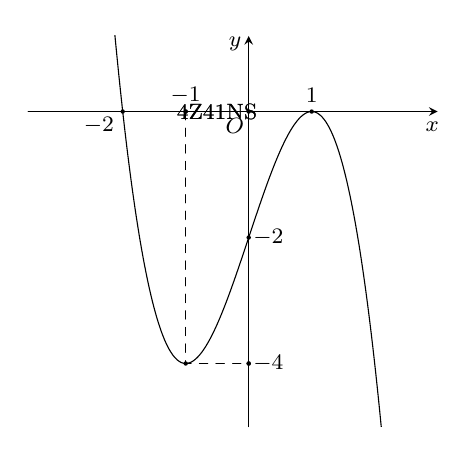
\begin{tikzpicture}[scale=.8, font=\footnotesize, line join=round, line cap=round, >=stealth]
    %hidden: VM005
			\def \xmin{-3.5}\def \xmax{3}\def \ymin{-5}\def \ymax{1.2} 
			\draw[->] (\xmin,0)--(\xmax,0) node[shift=(-110:0.2)] {$x$};
			\draw[->] (0,\ymin)--(0,\ymax) node[shift=(-150:0.2)] {$y$};
			\fill (0,0) node{\href{4Z41NS}{\tiny \phantom{4Z41NS}}} circle(1pt) node[shift=(-135:0.25)]{$O$};
			\fill (-2,0) circle(1pt) node[shift=(-150:0.35)]{$-2$};
			\fill (-1,0) circle(1pt) node[shift=(90:0.2)]{$-1$};
			\fill (1,0) circle(1pt) node[shift=(90:0.2)]{$1$};
			\fill (0,-4) circle(1pt) node[shift=(0:0.25)]{$-4$};
			\fill (0,-2) circle(1pt) node[shift=(0:0.25)]{$-2$};
			\fill (-1,-4) circle (1pt) (0,-4) circle (1pt) (-1,0) circle (1pt);
			\draw[dashed] (-1,0)-- (-1,-4) -- (0,-4);
			\clip (\xmin,\ymin) rectangle (\xmax,\ymax); 
			\draw[smooth,samples=100,domain=\xmin:\xmax] plot({\x}, {-\x*\x*\x + 3*\x - 2});
    \node at (0,0){\href{4Z41NS}{\tiny \phantom{4Z41NS}}};
		\end{tikzpicture}
		}
	\loigiai{
		Dựa vào đồ thị hàm số, ta thấy giá trị nhỏ nhất của hàm số trên đoạn $[-1;1]$ bằng $-4$ và đạt được khi $x=-1$.
	}
\end{ex}

\begin{ex}%[Dự án 4430CC-VN-MT-15]%[2-KS-15-SoHue-L1-2026,VM036,TV013]%[2H2N2-2]
	Trong không gian $Oxyz$, cho điểm $A(2;1;-2)$ và điểm $B(-4;3;4)$. Tọa độ trung điểm $M$ của đoạn $AB$ là
	\choice
		{$(3;2;3)$}
		{$(-2;2;2)$}
		{$(-2;-2;2)$}
		{\True $(-1;2;1)$}
	\loigiai{
		Vì $M$ là trung điểm của đoạn thẳng $AB$ nên tọa độ của điểm $M$ là $\left(\dfrac{2+(-4)}{2}; \dfrac{1+3}{2};\dfrac{-2+4}{2}\right)$, suy ra $M(-1;2;1)$.
	}
\end{ex}

\begin{ex}%[Dự án 51UG5W-VN-MT-15]%[2-KS-15-SoHue-L1-2026,VM036,TV013]%[0D0H2-2]
	Gieo một con xúc xắc cân đối và đồng chất một lần. Tính xác suất để xúc xắc xuất hiện mặt có số chấm là một số chia hết cho $3$.
	\choice
		{$\dfrac{1}{4}$}
		{$\dfrac{1}{2}$}
		{\True $\dfrac{1}{3}$}
		{$\dfrac{1}{6}$}
	\loigiai{
		Không gian mẫu của phép thử gieo xúc xắc một lần là $\Omega=\{1;2;3;4;5;6\}$.\\
		Suy ra $n(\Omega)=6$.\\
		Gọi $A$ là biến cố: \lq\lq Xúc xắc xuất hiện mặt có số chấm chia hết cho $3$\rq\rq.\\
		Các kết quả thuận lợi cho $A$ là $A=\{3;6\}$.\\
		Suy ra $n(A)=2$.\\
		Vậy xác suất của biến cố $A$ là $\mathrm{P}(A)=\dfrac{n(A)}{n(\Omega)}=\dfrac{2}{6}=\dfrac{1}{3}$.
	}
\end{ex}

\begin{ex}%[Dự án 4AWZ7D-VN-MT-15]%[2-KS-15-SoHue-L1-2026,VM036,TV013]%[2D4N1-2]
	Xác định họ các nguyên hàm của hàm số $f(x)=2x^2$.
	\choice
		{$6x^3+C$}
		{$\dfrac{x^3}{3}+C$}
		{$x^3+C$}
		{\True $\dfrac{2x^3}{3}+C$}
	\loigiai{
		Họ các nguyên hàm của hàm số $f(x)=2x^2$ là
		\[\displaystyle\int f(x) \mathrm{\,d}x=\displaystyle\int 2x^2\mathrm{\,d}x=2\cdot \dfrac{x^3}{3}+C=\dfrac{2x^3}{3}+C.\]
	}
\end{ex}

\begin{ex}%[Dự án 37M4HT-VN-MT-15]%[2-KS-15-SoHue-L1-2026,VM036,TV013]%[1H8N1-2]
	\immini[thm]{Cho hình chóp $S.ABCD$ có đáy $ABCD$ là hình chữ nhật và $SA \perp (ABCD)$. Đường thẳng $SA$ \textbf{không} vuông góc với đường thẳng nào trong các đường thẳng dưới đây?
		\choice[2]
			{$AC$}
			{$AB$}
			{$BD$}
			{\True $SC$}}{
		\begin{tikzpicture}[scale=1, font=\footnotesize, line join=round, line cap=round, >=stealth]
    %hidden: VM005
			\tikzset{declare function={a=3; b=1.8; h=3;}}
			\path (0,0) coordinate (A)
				(a,0) coordinate (D)
				(-150:b) coordinate (B)
				($(B)+(D)$) coordinate (C)
				(0,h) coordinate (S);
			\path pic[draw,angle radius=5pt]{right angle=B--A--S};
			\path pic[draw,angle radius=5pt]{right angle=D--A--S};
			\draw[dashed] (B)--(A)--(D)
				(A)--(C)
				(A)--(S);
			\draw (S)--(B)--(C)--(D)--cycle (S)--(C);
			\foreach \t/\g in {A/145,B/-90,C/-90,D/90,S/90}{
			\fill (\t) circle (1pt) node[shift={(\g:9pt)},font=\scriptsize]{$\t$};
			}
    \node at (0,0){\href{37M4HT}{\tiny \phantom{37M4HT}}};
		\end{tikzpicture}}
	\loigiai{
		Vì $SA\perp (ABCD)$ và $AC$, $AB$, $BD$ đều nằm trong $(ABCD)$ nên $SA \perp AC$, $SA\perp AB$, $SA \perp BD$.\\
		Vì $\triangle SAC$ vuông tại $A$ nên $\widehat{ASC}$ là góc nhọn.\\
		Suy ra $SA$ không vuông góc với $SC$.
	}
\end{ex}

\begin{ex}%[Dự án 1LTN51-VN-MT-15]%[2-KS-15-SoHue-L1-2026,VM036,TV013]%[2D1N4-1]
	\immini[thm]{Cho hàm số $y=\dfrac{ax+b}{cx+d}$ có đồ thị như hình vẽ bên. Xác định tiệm cận đứng của đồ thị hàm số hàm số đã cho.
		\choice[2]
			{$x = 1$}
			{$y = -1$}
			{\True $x = -1$}
			{$y = 1$}
		}{\begin{tikzpicture}[scale=.7, font=\footnotesize, line join=round, line cap=round, >=stealth]
    %hidden: VM005
			\def \xmin{-5.5}\def \xmax{3.5}\def \ymin{-5}\def \ymax{3} 
			\draw[->] (\xmin,0)--(\xmax,0) node[shift=(110:0.2)] {$x$};
			\draw[->] (0,\ymin)--(0,\ymax) node[shift=(-30:0.2)] {$y$};
			\fill (0,0) node{\href{1LTN51}{\tiny \phantom{1LTN51}}} circle(1pt) node[shift=(-45:0.25)]{$O$}; 
			\fill (-3,0) circle(1pt) node[shift=(90:0.2)]{$-3$}; 
			\fill (-1,0) circle(1pt) node[shift=(150:0.35)]{$-1$}; 
			\fill (1,0) circle(1pt) node[shift=(90:0.2)]{$1$}; 
			\fill (0,-2) circle(1pt) node[shift=(0:0.25)]{$-2$}; 
			\fill (0,-1) circle(1pt) node[shift=(-30:0.35)]{$-1$}; 
			\fill (0,1) circle(1pt) node[shift=(0:0.2)]{$1$}; 
			\fill (-3,-2) circle (1pt);
			\draw[dashed] (-3,0) -- (-3,-2) -- (0,-2);
			\clip (\xmin,\ymin) rectangle (\xmax,\ymax);
			\draw[smooth,samples=100,domain=\xmin:-1.1] plot (\x, {(-\x+1)/(\x+1)});
			\draw[smooth,samples=100,domain=-0.9:\xmax] plot(\x, {(-\x+1)/(\x+1)});
			\draw[smooth,samples=100,domain=\xmin:\xmax] plot(\x,{-1}); 
			\draw[smooth,samples=100,domain=\ymin:\ymax] plot({-1},\x);  
    \node at (0,0){\href{1LTN51}{\tiny \phantom{1LTN51}}};
		\end{tikzpicture}
		}
	\loigiai{
		Dựa vào đồ thị hàm số, ta có $\lim\limits_{x\to-1^+}y=+\infty$ và $\lim\limits_{x\to-1^-}y=-\infty$.\\
		Do đó, đồ thị hàm số có tiệm cận đứng là đường thẳng $x=-1$.
	}
\end{ex}

\Closesolutionfile{ans}
\cauds
\Opensolutionfile{ans}[ans/ans\currfilebase-Phan-II]
\begin{ex}%[Dự án 4RCOGW-VN-MT-15]%[2-KS-15-SoHue-L1-2026,TV035]%[2D4H2-6]
	\immini[thm]{Người ta muốn tạo một giá đỡ bằng sắt bên cạnh một bức tường có hình dạng là đoạn cong $BDN$ như hình vẽ bên, giá đỡ được gắn với tường bằng ba thanh sắt $AB$, $CD$, $MN$ cùng vuông góc với tường ($A$, $C$, $M$ thẳng hàng). Giá đỡ được xem như một phần của đồ thị hàm số $y=\log x$ trong mặt phẳng tọa độ $(Oxy)$ với trục tung trùng với hình chiếu vuông góc của giá đỡ lên mặt tường (đơn vị trên trục tính bằng mét). Biết $AB=10$\,cm, $AM=1{,}4$\,m và độ dài phần đồ thị của hàm số $y=f(x)$ liên tục trên đoạn $[a; b]$ được tính theo công thức $L = \displaystyle \int\limits_{a}^{b} \sqrt{1 + [f'(x)]^2} \mathrm{\,d}x$. 
		}{
		\begin{tikzpicture}[font=\footnotesize, line join=round, line cap=round, >=stealth,scale=0.65]
    %hidden: VM005
			% Vẽ tường bên trái (tô đậm)
			% \fill[pattern=north east lines] (-0.5,0) rectangle (0,5);
			%%%%%%%%%%%%%%%%%%%%%%%%%%%
			\coordinate (A) at (0,0);
			\coordinate (B) at (0.4,0);
			\coordinate (C) at (0,3);
			\coordinate (M) at (0,6);
			\coordinate (D) at (1.6,3);
			\coordinate (N) at (5,6);
			%%%%%%%%%%%%%%%%%%%%%%%%%%%
			\fill[pattern=north east lines,opacity=.5] (A)--(M)--($(M)-(1,0)$)--($(A)-(1,0)$)--cycle;
			\draw (A)--(C) -- (M) (M) -- (N) (C) -- (D) (A) -- (B);
			%%%%%%%%%%%%%%%%%%%%%%%%%%%
			\foreach \x/\pos in {A/-90,M/90,C/45,B/0,D/0,N/0} \fill (\x) circle(1pt) node[{shift=(\pos:0.25)}]{$\x$}; 
			%%%%%%%%%%%%%%%%%%%%%%%%%%%%%%%%%%%%%
			% Vẽ đường cong từ B đến N
			\draw (B) .. controls (0.61,1.29) and (1.29,2.45) .. (D);
			\draw (D) .. controls (2.61,4.31) and (3.77,5.49) .. (N);
			%%%%%%%%%%%%%%%%%%%%%%%%%%%%%%%%%%%%%
    \node at (0,0){\href{4RCOGW}{\tiny \phantom{4RCOGW}}};
		\end{tikzpicture}
		}
		\choiceTF
			{\True Đạo hàm của hàm số $y=\log x$ là $y' = \dfrac{1}{x \ln 10}$}
	{\True Trong mặt phẳng tọa độ $(Oxy)$, điểm $B$ có hoành độ bằng $0{,}1$}
	{Trong mặt phẳng tọa độ $(Oxy)$, điểm $N$ có tung độ bằng $1{,}4$}
	{\True Độ dài giá đỡ bằng $2{,}97$ mét (kết quả được làm tròn đến hàng phần trăm)}
	\loigiai{
		\begin{itemchoice}
			\itemch Ta có $y' = (\log x)' = \dfrac{1}{x \ln 10}$. 
			\itemch Do $AB=10$\,cm $=0{,}1$\,m nên hoành độ của điểm $B$ là $0{,}1$. 
			\itemch Do $B$ thuộc đồ thị hàm số $y=\log x$ nên ta có 
			\[
			y_B = \log 0{,}1 \Leftrightarrow y_B =-1. 
			\]
			Suy ra, điểm $A$ cách gốc tọa độ $O$ một khoảng bằng $1$\,m. \\
			Do $AM=1{,}4$\,m nên tung độ của điểm $M$ bằng $0{,}4$. \\
			Suy ra tung độ của điểm $N$ là $0{,}4$.  
			\itemch Do điểm $N$ thuộc đồ thị hàm số $y=\log x$ và tung độ của $N$ bằng $0{,}4$ nên ta có 
			\[
			\log x_N = 0{,}4 \Leftrightarrow x_N = 10^{0{,}4}. 
			\]
			Vậy độ dài $L$ của giá đỡ là 
			\[
			L = \displaystyle \int\limits_{0{,}1}^{10^{0{,}4}} \sqrt{1 + \left(\dfrac{1}{x \ln 10}\right)^2} \mathrm{d}x \approx 2{,}97 \text{ (m)}. 
			\]
		\end{itemchoice}
	}
\end{ex}

\begin{ex}%[Dự án 2C5C4B-VN-MT-15]%[2-KS-15-SoHue-L1-2026, VM006]%[2D6V2-2]
	Một hộp có $12$ viên bi gồm $5$ bi xanh, $6$ bi đỏ và $1$ bi vàng. Hai bạn tên Xanh và Đỏ được trọng tài mời chơi trò chơi bốc bi ngẫu nhiên từ hộp (bi đã lấy ra không bỏ lại vào hộp). Đầu tiên trọng tài bốc một viên bi, nếu là bi xanh hoặc bi đỏ thì dừng bốc, nếu là bi vàng thì trọng tài bốc thêm một viên nữa rồi dừng bốc. Sau khi trọng tài dừng bốc, viên bi trọng tài bốc màu nào thì bạn có tên màu đó sẽ được bốc một viên và ngay sau đó trò chơi dừng lại. Người chơi bốc được viên bi có màu trùng với tên của mình sẽ là người thắng cuộc, còn nếu bốc được viên bi có màu khác với tên mình sẽ bị thua cuộc.
	\choiceTF 
		{\True Xác suất để trọng tài bốc được bi vàng trong lần bốc đầu tiên là $\dfrac{1}{12}$} 
		{Giả sử rằng ở lần bốc đầu tiên trọng tài bốc được bi xanh. Khi đó xác suất để bạn Xanh thắng là $\dfrac{5}{11}$} 
		{\True Giả sử rằng ở lần bốc đầu tiên trọng tài bốc được bi vàng và bốc tiếp được bi đỏ. Khi đó xác suất để bạn Xanh thắng là $\dfrac{1}{2}$} 
		{Xác suất để bạn Đỏ thắng là $\dfrac{6}{11}$} 
	\loigiai{
		\begin{itemchoice} 
			\itemch Xác suất để trọng tài bốc được bi vàng trong lần đầu tiên là $\dfrac{1}{12}$.
			\itemch Nếu lần bốc đầu tiên trọng tài bốc được bi xanh. Khi đó trong hộp còn $4$ bi xanh, $6$ bi đỏ và $1$ bi vàng xác suất để bạn Xanh thắng (bốc được bi xanh) là $\dfrac{4}{11}$.
			\itemch Nếu lần bốc đầu tiên trọng tài bốc được bi vàng và bốc tiếp được bi đỏ. Khi đó trong hộp còn $5$ bi xanh, $5$ bi đỏ xác suất để bạn Xanh thắng (bạn Đỏ bốc được bi xanh) là $\dfrac{5}{10}=\dfrac{1}{2}$.
			\itemch Theo luật chơi như trên, sẽ luôn có bạn thắng, bạn còn lại thua và không có kết quả cả hai cùng thua hoặc hòa.\\
			Để tính xác suất của Đỏ thắng, ta tính xác suất của Xanh thắng và xét các trường hợp sau:
			\begin{enumerate}[\it TH 1:]
				\item Lần đầu tiên trọng tài bốc được bi xanh, xác suất là $\dfrac{5}{12}$.\\
				Nếu lần bốc đầu tiên trọng tài bốc được bi xanh, xác suất để bạn Xanh thắng là $\dfrac{4}{11}$.\\
				Suy ra xác xuất lần bốc đầu tiên trọng tài bốc được bi xanh và bạn Xanh thắng là $\dfrac{5}{12}\cdot\dfrac{4}{11}=\dfrac{5}{33}$.
				\item Lần đầu tiên trọng tài bốc được bi đỏ, xác suất là $\dfrac{6}{12}=\dfrac{1}{2}$.\\
				Nếu lần bốc đầu tiên trọng tài bốc được bi đỏ, xác suất để bạn Xanh thắng là $\dfrac{6}{11}$.\\
				Suy ra xác xuất lần bốc đầu tiên trọng tài bốc được bi đỏ và bạn Xanh thắng là \[\dfrac{1}{2}\cdot\dfrac{6}{11}=\dfrac{3}{11}.\]
				\item Lần bốc đầu tiên trọng tài bốc được bi vàng và bốc tiếp được bi đỏ, xác suất là \[\dfrac{1}{12}\cdot\dfrac{6}{11}=\dfrac{1}{22}.\]
				Nếu lần bốc đầu tiên trọng tài bốc được bi vàng và bốc tiếp được bi đỏ, xác suất để bạn Xanh thắng là $\dfrac{5}{10}=\dfrac{1}{2}$.\\
				Suy ra xác xuất lần bốc đầu tiên trọng tài bốc được bi vàng, bốc tiếp được bi đỏ và Xanh thắng là $\dfrac{1}{22}\cdot\dfrac{1}{2}=\dfrac{1}{44}$.
				\item Lần bốc đầu tiên trọng tài bốc được bi vàng và bốc tiếp được bi xanh, xác suất là $\dfrac{1}{12}\cdot\dfrac{5}{11}=\dfrac{5}{132}$.\\
				Nếu lần bốc đầu tiên trọng tài bốc được bi vàng và bốc tiếp được bi xanh, xác suất để bạn Xanh thắng là $\dfrac{4}{10}=\dfrac{2}{5}$.\\
				Suy ra xác xuất lần bốc đầu tiên trọng tài bốc được bi vàng, bốc tiếp được bi xanh và Xanh thắng là $\dfrac{5}{132}\cdot\dfrac{2}{5}=\dfrac{1}{66}$.
			\end{enumerate}
			Do đó xác xuất để Xanh thắng là $\dfrac{5}{33}+\dfrac{3}{11}+\dfrac{1}{44}+\dfrac{1}{66}=\dfrac{61}{132}$.\\
			Vậy xác suất để Đỏ thắng (Xanh thua) là $1-\dfrac{61}{132}=\dfrac{71}{132}$.
		\end{itemchoice} 
	}
\end{ex}

\begin{ex}%[Dự án 1JP07M-VN-MT-15]%[2-KS-15-SoHue-L1-2026, VM006]%[2D1H5-4]
	Cho hàm số $y=f(x)=\dfrac{x^2-5x+4}{x-5}$ với $x\neq 5$.
	\choiceTF 
		{\True $f'(x)=1-\dfrac{4}{(x-5)^2}$ với mọi $x\neq 5$} 
		{\True Đồ thị hàm số cắt trục hoành tại hai điểm phân biệt} 
		{\True Hàm số đạt cực đại tại $x=3$} 
		{Giá trị cực tiểu bằng $3$} 
	\loigiai{
		\begin{itemchoice} 
			\itemch Với $x\neq 5$, ta có $y=f(x)=x+\dfrac{4}{x-5}\Rightarrow f'(x)=1-\dfrac{4}{(x-5)^2}$.
			\itemch Với $x\neq 5$, xét phương trình hoành độ giao điểm của đồ thị hàm số với trục hoành, ta được
			\[
			\dfrac{x^2-5x+4}{x-5}=0\Leftrightarrow x^2-5x+4=0\Leftrightarrow\hoac{&x=1\\&x=4.}
			\]
			Cả hai giá trị $x=1$; $x=4$ đều thỏa điều kiện.\\
			Vì phương trình có $2$ nghiệm phân biệt nên đồ thị hàm số cắt trục hoành tại hai điểm phân biệt.
			\itemch Ta có $y'=f'(x)=1-\dfrac{4}{(x-5)^2}=\dfrac{x^2-10x+21}{(x-5)^2}$.\\
			Xét $f'(x)=0\Leftrightarrow \dfrac{x^2-10x+21}{(x-5)^2}=0\Leftrightarrow\hoac{&x=7 \\&x=3.}$\\
			Bảng biến thiên của hàm số $y=f(x)$ như sau:
			\begin{center}
				\begin{tikzpicture}
    %hidden: VM005
					\tkzTabInit[nocadre=true,lgt=1.2,espcl=2.5,deltacl=0.5]
					{$x$/0.7,$f’(x)$/0.7,$f(x)$/2}
					{$-\infty$,$3$,$5$,$7$,$+\infty$}
					\tkzTabLine{,+,0,-,d,-,0,+,}
					\tkzTabVar{-/$-\infty$,+/$1$,-D+/$-\infty$/$+\infty$,-/$9$,+/$+\infty$}
    \node at (T11){\href{1JP07M}{\tiny \phantom{1JP07M}}};
				\end{tikzpicture}
			\end{center}
			Dựa vào bảng biến thiên, hàm số đạt cực đại tại $x=3$.
			\itemch Dựa vào bảng biến thiên, giá trị cực tiểu của hàm số là $9$.
		\end{itemchoice} 
	}
\end{ex}

\begin{ex}%[Dự án 29NBVX-VN-MT-15]%[2-KS-15-SoHue-L1-2026,TV035]%[2H5H2-5]
	Trong không gian $Oxyz$, cho điểm $A (1; 2; 3)$ và điểm $B (2; 3; 4)$. Gọi $M$ là giao điểm của đường thẳng đi qua hai điểm $A$, $B$ với mặt phẳng $(Oxy)$, $N$ thuộc trục $Oz$ sao cho $AN$ vuông góc với $AB$. 
	\choiceTF
		{\True $\overrightarrow{AB} = (1; 1; 1)$}
		{Hoành độ của điểm $M$ bằng $-1$}
		{$MA = - 3 AB$}
		{\True $\tan \widehat{NMB} = \dfrac{\sqrt{42}}{9}$}
	\loigiai{
		\begin{itemchoice}
			\itemch Ta có $\overrightarrow{AB} = (1; 1; 1)$. 
			\itemch Đường thẳng $AB$ đi qua điểm $A (1; 2; 3)$, nhận $\overrightarrow{AB}$ làm một vectơ chỉ phương có phương trình tham số là $\heva{& x = 1 + t \\ & y = 2 + t \\ & z = 3 + t}$ với $t \in \mathbb{R}$. \\
			Phương trình mặt phẳng $(Oxy)$ là $z=0$. \\ 
			Gọi $M$ là giao điểm của $AB$ và mặt phẳng $(Oxy)$. \\ 
			Do $M \in AB$ nên $M (1+t; 2+t; 3+t)$. \\ 
			Do $M \in (Oxy)$ nên $t+3=0 \Leftrightarrow t=-3$. \\
			Suy ra, $M (-2; -1; 0)$. \\
			Vậy hoành độ của điểm $M$ bằng $-2$. 
			\itemch $\overrightarrow{MA} = (3; 3; 3) \Rightarrow MA = 3 \sqrt{3}$. \\
			$\overrightarrow{AB} = (1; 1; 1) \Rightarrow AB = \sqrt{3}$. \\
			Vậy suy ra $MA = 3 AB$. 
			\itemch Do $N \in Oz \Rightarrow N (0; 0; z)$. \\
			Ta có $\overrightarrow{AN} = (-1; -2; z-3)$. \\
			Do $AN \perp AB \Rightarrow \overrightarrow{AN} \cdot \overrightarrow{AB} = 0 \Leftrightarrow -1 -2 + (z-3) =0 \Leftrightarrow z = 6$. \\
			Vậy $N (0; 0; 6)$. \\
			Ta có $\overrightarrow{MN} = (2; 1; 6)$, $\overrightarrow{MB} = (4; 4; 4)$. \\
			Suy ra $\cos \widehat{NMB} = \cos \left(\overrightarrow{MN}, \overrightarrow{MB}\right) = \dfrac{2 \cdot 4 + 1 \cdot 4 + 6 \cdot 4}{\sqrt{2^2 + 1^2 + 6^2} \cdot \sqrt{4^2 + 4^2 + 4^2}} = \dfrac{3 \sqrt{123}}{41}$. \\
			Do $\cos \widehat{NMB} >0$ nên $\widehat{NMB}$ là góc nhọn và $\tan \widehat{NMB} >0$. \\
			Ta có 
			\[
			1 + \tan^2 \widehat{NMB} = \dfrac{1}{\cos^2 \widehat{NMB}} \Rightarrow \tan^2 \widehat{NMB} = \dfrac{1}{\cos^2 \widehat{NMB}} - 1 = \dfrac{14}{27} \Rightarrow \tan \widehat{NMB} = \dfrac{\sqrt{42}}{9}. 
			\]
		\end{itemchoice}
	}
\end{ex}

\Closesolutionfile{ans}
\caukq
\Opensolutionfile{ans}[ans/ans\currfilebase-Phan-III]
\begin{ex}%[Dự án 5M9QY0-VN-MT-15]%[2-KS-15-SoHue-L1-2026,TV015]%[0D7V3-6]
	Một hộ sản xuất và kinh doanh một mặt hàng A, biết rằng chi phí để sản xuất $x$ kg ($x > 0$) mặt hàng A là $\dfrac{2x^2+x}{x+1}$ (đơn vị triệu đồng), trong lúc đó bán ra mỗi kg là $3$ triệu đồng. Hỏi cần sản xuất bao nhiêu kg mặt hàng A để lợi nhuận đạt $15$ triệu đồng {\it(kết quả làm tròn đến hàng phần chục)}.
	\par\shortans{$14{,}1$}
	\loigiai{
		Giá bán mỗi kg là $3$ triệu đồng, nên doanh thu khi bán $x$ kg là $R(x) = 3x$ (triệu đồng). \\
		Chi phí để sản xuất $x$ kg mặt hàng A là $C(x) = \dfrac{2x^2+x}{x+1}$ (triệu đồng). \\
		Lợi nhuận thu được khi sản xuất và kinh doanh $x$ kg mặt hàng A là
		\begin{align*}
			P(x) &= R(x) - C(x) \\
			&= 3x - \dfrac{2x^2+x}{x+1}\\
			&= \dfrac{x^2+2x}{x+1}.
		\end{align*}
		Để lợi nhuận đạt $15$ triệu đồng, thì
		\begin{eqnarray*}
			&&P(x)=15\\
			&\Leftrightarrow&\dfrac{x^2+2x}{x+1} = 15\\
			&\Rightarrow&x^2 - 13x - 15 = 0\\
			&\Rightarrow&\hoac{&x=\dfrac{13 + \sqrt{229}}{2}\\&x=\dfrac{13 - \sqrt{229}}{2}.}
		\end{eqnarray*}
		Vì $x > 0$, ta chọn $x = \dfrac{13 + \sqrt{229}}{2}\approx 14{,}1$\,(kg). \\
		Vậy cần sản xuất khoảng $14{,}1$ kg mặt hàng A để lợi nhuận đạt $15$ triệu đồng.
	}
\end{ex}

\begin{ex}%[Dự án 5B4FXE-VN-MT-15]%[2-KS-15-SoHue-L1-2026,VM021]%[1H8V5-4]
	Cho hình chóp cụt tam giác đều $ABC.MNP$ có đáy lớn là tam giác $ABC$ với độ dài cạnh bằng $6$, chiều cao của hình chóp cụt bằng $8$. Gọi $G$ là trọng tâm tam giác $MNP$. Tính khoảng cách giữa hai đường thẳng $AG$ và $BC$ \textit{(kết quả làm tròn đến hàng phần trăm)}.
	\par\shortans{$4{,}77$}
	\loigiai{
		\begin{center}
			\begin{tikzpicture}[scale=1.5, font=\footnotesize, line join=round, line cap=round,>=stealth]
    %hidden: VM005
				\pgfresetboundingbox
				\def \k{0.6};
				\path (0,0)coordinate (A) (4.5,0) coordinate (C) (3.5,-2) coordinate (B) ($(B)!0.5!(C)$) coordinate (I) ($(A)!2/3!(I)$) coordinate (O) (0,3) coordinate (h) ($(O)+(h)$) coordinate (S)
					($(A)!\k!(S)$) coordinate (M)
					($(B)!\k!(S)$) coordinate (N)
					($(C)!\k!(S)$) coordinate (P)
					;
				\path ($(N)!0.5!(P)$) coordinate (I');
				\path ($(M)!2/3!(I')$) coordinate (G)
					($(A)!0.7!(G)$) coordinate (H);
				\draw (M)--(A)--(B)--(C)--(P)--cycle (N)--(P) (M)--(N)--(B)  (M)--(I')--(I);
				\draw[dashed] (I)--(A)--(C) (O)--(G) (I)--(H) (A)--(G) (G)--(I);
				\foreach \p/\g in {A/150,B/-60,C/30, M/150, N/-30, P/30, I/0,O/-90, I'/0, G/20,H/120} \fill (\p) circle(1pt)+(\g:0.3) node{$\p$};
				\path pic[angle radius=3mm,draw=black,angle eccentricity=1] {right angle = G--O--A};
    \node at (0,0){\href{5B4FXE}{\tiny \phantom{5B4FXE}}};
			\end{tikzpicture}
		\end{center}
		Gọi $I$ và $I'$ lần lượt là trung điểm của $BC$ và $NP$. \\
		Khi đó $\heva{&BC \perp AI\\ &BC \perp II'} \Rightarrow BC \perp (AMI'I)$.\\
		Gọi $H$ thuộc $AG$ sao cho $IH \perp AG$.\\
		Khi đó $\heva{&IH \perp AG, IH \cap AG = H \\
		&IH \perp BC, IH \cap BC = I.}$\\
		Suy ra $IH$ là đoạn vuông góc chung của $AG$ và $BC$. \\
		Vậy $\mathrm{d}(AG,BC)=IH$.\\
		Gọi $O$ là trọng tâm tam giác $ABC$, khi đó $GO \perp (ABC)$, suy ra $GO=8$.\\
		Lại có $AI=\dfrac{AB\sqrt{3}}{2}=\dfrac{6\sqrt{3}}{2}=3\sqrt{3}$ và $AO=\dfrac{2}{3}\cdot AI=2\sqrt{3}$.\\
		Ta có $AG=\sqrt{GO^2+AO^2}=\sqrt{8^2+\left(2\sqrt{3}\right)^2}=2\sqrt{19}$.\\
		Xét tam giác $AGI$ ta có
		\allowdisplaybreaks
		\begin{eqnarray*}
			S_{AGI}&=&\dfrac{1}{2}\cdot IH \cdot AG = \dfrac{1}{2}\cdot GO \cdot AI \\
			&\Leftrightarrow& IH=\dfrac{GO \cdot AI}{AG}=\dfrac{8 \cdot 3\sqrt{3}}{2\sqrt{19}}=\dfrac{12\sqrt{57}}{19}\approx 4{,}77.
		\end{eqnarray*}
	}
\end{ex}

\begin{ex}%[Dự án 525W4N-VN-MT-15]%[2-KS-15-SoHue-L1-2026,TV015]%[2D4V2-6]
	An và Bình rất giỏi Toán, cùng tham gia một trò chơi, đầu tiên An bốc ngẫu nhiên một thẻ từ hộp thứ nhất chứa sáu thẻ giống nhau được đánh số từ $1$ đến $6$, tiếp theo Bình bốc ngẫu nhiên một thẻ từ hộp thứ hai chứa bốn thẻ giống nhau được đánh số từ $1$ đến $4$. Gọi số An bốc được là $a$ và số của Bình là $b$, sau đó hai người cùng tính giá trị của tích phân $I = \displaystyle\int\limits_{0}^{a} x^b \mathrm{\,d}x$. Nếu kết quả $I$ là một số nguyên thì An thắng, ngược lại Bình thắng. Tính xác suất An thắng cuộc {\it (kết quả làm tròn đến hàng phần trăm)}.
	\par\shortans{$0{,}38$}
	\loigiai{
		An bốc một thẻ từ hộp thứ nhất có các số $a \in \{1, 2, 3, 4, 5, 6\}$. Có $6$ khả năng. \\
		Bình bốc một thẻ từ hộp thứ hai có các số $b \in \{1, 2, 3, 4\}$. Có $4$ khả năng. \\
		Tổng số cặp $(a,b)$ có thể xảy ra là $n\left(\Omega\right)=6 \cdot 4 = 24$.\\
		Vì $b \ge 1$, ta có
		\[I = \displaystyle\int\limits_{0}^{a} x^b \mathrm{\,d}x=\dfrac{a^{b+1}}{b+1}.\]
		Gọi $A$ là biến cố bạn An thắng cuộc.\\
		Ta cần tìm các cặp $(a,b)$ sao cho $I=\dfrac{a^{b+1}}{b+1}$ là một số nguyên.\\
		Liệt kê tất cả các khả năng có thể xảy ra
		\begin{center}
			\renewcommand{\arraystretch}{2} % Điều chỉnh số này để vừa ý
			\begin{tabular}{|c|c|c|c|c|}
				\hline
				& $b=1$ & $b=2$ & $b=3$ & $b=4$ \\
				\hline
				$a=1$ & $I=\dfrac{1}{2}$ & $I=\dfrac{1}{3}$ & $I=\dfrac{1}{4}$ & $I=\dfrac{1}{5}$ \\
				\hline
				$a=2$ & $I=2$ & $I=\dfrac{8}{3}$ & $I=4$ & $I=\dfrac{32}{5}$ \\
				\hline
				$a=3$ & $I=\dfrac{9}{2}$ & $I=9$ & $I=\dfrac{81}{4}$ & $I=\dfrac{243}{5}$ \\
				\hline
				$a=4$ & $I=8$ & $I=\dfrac{64}{3}$ & $I=64$ & $I=\dfrac{1\,024}{5}$ \\
				\hline
				$a=5$ & $I=\dfrac{25}{2}$ & $I=\dfrac{125}{3}$ & $I=\dfrac{625}{4}$ & $I=625$ \\
				\hline
				$a=6$ & $I=18$ & $I=72$ & $I=324$ & $I=\dfrac{7\,776}{5}$ \\
				\hline
			\end{tabular}
		\end{center}
		Các cặp $(a,b)$ thỏa mãn $I\in\mathbb{Z}$ là $(2,1)$, $(2,3)$, $(3,2)$, $(4,1)$, $(4,3)$, $(5,4)$, $(6,1)$, $(6,2)$, $(6,3)$.\\ Suy ra $n(A)=9$.\\
		Vậy $\mathrm{P}(A)=\dfrac{n(A)}{n\left(\Omega\right)}=\dfrac{9}{24}\approx 0{,}38$.
	}
\end{ex}

\begin{ex}%[Dự án 20Y0IT-VN-MT-15]%[2-KS-15-SoHue-L1-2026,TV015]%[0H4V3-2]
	Dòng Hương hiền hòa trong xanh, lững lờ trôi giữa lòng thành phố Huế cổ kính và mộng mơ. Nhìn từ trên cao, hai bờ sông trải dài như hai đường thẳng song song. Cột cờ Phu Văn Lâu sừng sững cao $54{,}5$\,mét như là một chứng tích hào hùng của lịch sử. Biết rằng hai bờ sông cách nhau $400$\,mét và chân cột cờ (hình chiếu vuông góc của đỉnh cột cờ xuống mặt đất) nằm cách mép sông gần nhất một khoảng $200$\,mét. Có hai bạn học sinh đứng ở hai bờ sông, bạn học sinh A ở cùng bờ với cột cờ nhìn đỉnh cột cờ so với mặt đất một góc $\alpha$ với $\tan \alpha = 0{,}1$ và bạn học sinh B đứng ở bờ bên kia nhìn đỉnh cột cờ so với mặt đất một góc $\beta$ với $\tan \beta = 0{,}07$. Hỏi hai bạn học sinh cách nhau xa nhất là bao nhiêu mét? {\it (Giả sử rằng mặt đất là bằng phẳng và tầm mắt hai bạn học sinh ngang với mặt đất, kết quả làm tròn đến hàng đơn vị)}.
	\begin{center}
		\begin{tikzpicture}[scale=0.7, font=\footnotesize, line join=round, line cap=round, >=stealth]
    %hidden: VM005
			\tikzset{declare function={h=3;goca=-10;gocb=-25;ds=-3*h;}}
			\path
				(0,0) coordinate (H)
				(0,h) coordinate (S)
				(goca:2*h) coordinate (A)++(-goca+10:ds)coordinate (bA)
				(gocb:3*h) coordinate (B)++(-goca+10:ds)coordinate (bB)
				($(bA)!1.2!(A)$)coordinate (Aa) ($(bB)!1.2!(B)$)coordinate (Bb);
			\pic[angle eccentricity=1.3,draw,angle radius=15pt]{angle= S--A--H}
			pic[angle eccentricity=1.2,draw,angle radius=28pt]{angle= S--B--H}
			pic[angle eccentricity=1.2,draw,angle radius=30pt]{angle= S--B--H};
			\fill[cyan!30,opacity=0.5] (bA)--(Aa)--(Bb)--(bB)--cycle;
			\draw[dashed] (A)--(H)--(B);
			\draw (H)--(S)node[left,midway]{Cột cờ}--(A) (S)--(B) (bA)--(Aa) (bB)--(Bb);
			\foreach \x/\pos in {A/90,B/-60,S/90,H/180} \fill (\x) circle(1pt) node[{shift=(\pos:0.25)}]{$\x$}; 
			\node[shift=(156:0.7)] at (A) {$\alpha$};
			\node[shift=(146.8:1.5)] at (B) {$\beta$};
    \node at (0,0){\href{20Y0IT}{\tiny \phantom{20Y0IT}}};
		\end{tikzpicture}
	\end{center}
	\par\shortans{$1\,080$}
	\loigiai{
		Tam giác $SHA$ vuông tại $H$ có $HA = \dfrac{HK}{\tan \alpha} = \dfrac{54{,}5}{0{,}1} = 545$\,mét.\\
		Tam giác $SHB$ vuông tại $H$ có $HB = \dfrac{HK}{\tan \beta} = \dfrac{54{,}5}{0{,}07} \approx 778{,}57$\,mét.\\
		Trên bờ sông có cột cờ, tồn tại hai điểm $A$ và $A'$ sao cho $HA=HA'$.\\ Gọi $M$ là trung điểm của $AA'$ suy ra $HM=200$\,mét.\\
		Trên bờ sông còn lại, tồn tại hai điểm $B$ và $B'$ sao cho $HB=HB'$.\\ Gọi $N$ là trung điểm của $BB'$ suy ra $MN=400$\,mét.\\
		Tham khảo hình vẽ
		\begin{center}
			\begin{tikzpicture}[scale=0.7, font=\footnotesize, line join=round, line cap=round, >=stealth]
    %hidden: VM005
				\tikzset{declare function={r=3;R=5;}}
				\path
					(0,0) coordinate (M)++(0,r-1)coordinate (H)
					(-R,0)coordinate (A') (R,0)coordinate (A)
					(0,-R+2) coordinate (N)++(r,0)coordinate (B)
					(N)++(-r,0)coordinate (B')
					($(B')!(A')!(B)$)coordinate (K);
				\foreach\x/\y/\z in {H/M/A,M/N/B,A'/K/N}{
				\path pic[draw,angle radius=5pt]{right angle=\x--\y--\z};}
				\draw[dashed] (A')--(H)--(A) (H)--(N) (B')--(H)--(B) (A')--(K)--(B');
				\draw (A)--(A') (B)--(B');
				\draw[red] (A')--(B);
				\foreach \x/\g in {A/0,B/0,A'/180,H/90,B'/-90,M/140,N/-90,K/-90}
				\fill (\x) circle (1pt)+(\g:12pt) node {$\x$};
    \node at (0,0){\href{20Y0IT}{\tiny \phantom{20Y0IT}}};
			\end{tikzpicture}
		\end{center}
		Như vậy, hai bạn học sinh A và B cách xa nhau nhất khi học sinh A ở điểm $A'$ và học sinh B ở điểm $B$ hoặc ngược lại.\\
		Gọi $K$ là hình chiếu vuông góc của điểm $A'$ trên đường thẳng $BB'$.\\
		Tam giác $HMA'$ vuông tại $M$ có $KN=MA'=\sqrt{HA'^2-HM^2}=\sqrt{545^2-200^2}\approx 507$\,m.\\
		Tam giác $HNB$ vuông tại $N$ có $NB=\sqrt{HB^2-HN^2}=\sqrt{(778{,}57)^2-(200+400)^2}\approx 496{,}2$\,mét
		Tam giác $A'KB$ vuông tại $K$ có
		\[A'B=\sqrt{A'K^2+KB^2}=\sqrt{400^2+(507+496{,}2)^2}\approx 1\,080\text{( mét)}.\]
	}
\end{ex}

\begin{ex}%[Dự án 16DSGO-VN-MT-15]%[2-KS-15-SoHue-L1-2026,VM021]%[1D2C3-8]
	Đất sét là một dạng vật chất đặc và mềm, có thể tạo thành nhiều hình dạng khác nhau nhưng thể tích không đổi. Đầu tiên ta có một cục đất sét với thể tích $1\,000$\,cm$^3$, người ta nặn thành một khối lập phương đặc, sau đó khoét phần đất sét ở giữa để tạo thành một chậu không nắp (phần trong của chậu có dạng hình hộp chữ nhật) có độ dày bốn mặt bên và độ dày đáy bằng nhau và bằng $\dfrac{1}{10}$ độ dài cạnh của khối lập phương. Phần đất sét còn dư cũng được nặn thành một khối lập phương đặc và cũng khoét phần đất sét ở giữa để tạo thành một chậu không nắp với tỉ lệ giữa độ dày của các mặt và cạnh khối lập phương như trên. Cứ tiếp tục như vậy cho đến khi được $5$ cái chậu. Tính tổng thể tích nước mà $5$ chậu đó có thể chứa \textit{(đơn vị là cm$^3$, kết quả làm tròn đến hàng đơn vị)}.
	\par\shortans{$1\,272$}
	\loigiai{
		Gọi $V_n$ là thể tích của khối đất sét đặc (khối lập phương) ở bước thứ $n$. Ban đầu ta có $V_1 = 1\,000$.\\
		Giả sử khối lập phương ở bước $n$ có cạnh là $a$, khi đó $V_n = a^3$.\\
		Chậu không nắp được khoét ra có độ dày các mặt bên và đáy bằng $\dfrac{a}{10}$.\\
		Phần rỗng bên trong chậu (chính là lượng nước mà chậu chứa được) có dạng hình hộp chữ nhật với
		\begin{itemize}
			\item Độ dài cạnh đáy: $a - 2 \cdot \dfrac{a}{10} = \dfrac{4a}{5}$
			\item Chiều cao: $a - \dfrac{a}{10} = \dfrac{9a}{10}$
		\end{itemize}
		Thể tích phần rỗng (thể tích nước chậu thứ $n$ chứa được) là
		$W_n = \left(\dfrac{4a}{5}\right)^2 \cdot \dfrac{9a}{10} = \dfrac{72a^3}{125} = \dfrac{72}{125}V_n$.\\
		Phần đất sét được khoét ra (có thể tích đúng bằng phần rỗng) sẽ là lượng đất sét dư để nặn thành khối lập phương cho bước tiếp theo. Do đó, ta có
		$V_{n+1} = W_n = \dfrac{72}{125}V_n$.\\
		Với $V_1 = 1\,000$, thể tích nước chậu đầu tiên chứa được là
		$W_1 = \dfrac{72}{125} \cdot 1000 = 576$.\\
		Thể tích nước chậu thứ $n+1$ chứa được là
		$W_{n+1} = \dfrac{72}{125}V_{n+1} = \dfrac{72}{125}W_n$.\\
		Như vậy, dãy các thể tích nước $W_1$, $W_2$, $W_3$, $\dots$, $W_5$ lập thành một cấp số nhân có số hạng đầu $u_1 = W_1 = 576$ và công bội $q = \dfrac{72}{125}$.\\
		Tổng thể tích nước mà $5$ chậu có thể chứa chính là tổng $5$ số hạng đầu tiên của cấp số nhân này, khi đó
		\[
		W = 576 \cdot \dfrac{1 - \left(\dfrac{72}{125}\right)^5}{1 - \dfrac{72}{125}} \approx 1\,272 \text{ (cm}^3\text{)}.
		\]
	}
\end{ex}

\begin{ex}%[Dự án 57KY07-VN-MT-15]%[2-KS-15-SoHue-L1-2026,VM021]%[0D8V2-7]
	Hằng năm trước ngày Khai giảng năm học mới. Ủy ban nhân dân thành phố Huế giao Sở Giáo dục và Đào tạo tổ chức Lễ Tuyên dương học sinh dạt danh hiệu \lq\lq Học sinh danh dự toàn trường\rq\rq\ dành cho những học sinh xuất sắc nhất của mỗi trường phổ thông trên địa bàn thành phố. Trong Lễ Tuyên dương. Ban tổ chức vinh danh các học sinh theo lượt nhận, mỗi lượt có $10$ học sinh, với những lượt có $5$ học sinh nam và $5$ học sinh nữ thì Ban tổ chức muốn các học sinh này đứng thành một hàng mà nam nữ xen kẽ. Tuy nhiên khi xếp hàng với lượt có $5$ học sinh nam và $5$ học sinh nữ thì Ban tổ chức nhận thấy các học sinh này không đứng xen kẽ nhưng chỉ cần đổi chỗ hai học sinh nào đó thì được hàng có nam nữ đứng xen kẽ, cách xếp này gọi là \lq\lq cách xếp lỗi\rq\rq. Gọi $D$ là số \lq\lq cách xếp lỗi\rq\rq\ như trên, xác định giá trị của $\dfrac{D}{100}$.
	\par\shortans{$7\,200$}
	\loigiai{
		Số cách xếp $5$ nam và $5$ nữ đứng xen kẽ (gọi là cách xếp chuẩn) là: $2 \cdot 5! \cdot 5!$ cách (do có $2$ trường hợp nam hoặc nữ đứng đầu hàng).\\
		Một \lq\lq cách xếp lỗi\rq\rq\ là hàng có đúng $2$ vị trí sai giới tính. Để tạo ra một cách xếp lỗi, ta lấy một hàng chuẩn và đổi chỗ đúng $1$ học sinh nam với $1$ học sinh nữ. Khi đó, số cách chọn $1$ nam và $1$ nữ từ hàng chuẩn để đổi chỗ là $\mathrm{C}_5^1 \cdot \mathrm{C}_5^1 = 25$ cách.\\
		Vì mỗi \lq\lq cách xếp lỗi\rq\rq\ chỉ được tạo ra từ duy nhất một hàng chuẩn và một cặp đổi chỗ, áp dụng quy tắc nhân, ta có số cách xếp lỗi là
		\[ D = (2 \cdot 5! \cdot 5!) \cdot 25 = 720\,000. \]
		Vậy $\dfrac{D}{100} = 7\,200$.
	}
\end{ex}

\Closesolutionfile{ans}
\Closesolutionfile{ansbook}
\begin{indapan}
	{ans/ans\currfilebase}
\end{indapan}